%! Author = lili
%! Date = 5/4/26
Aus dem Intervall [0, 1] wird rein zufällig eine Zahl gezogen. Wir betrachten in dieser Aufgabe
nur die Nachkommastellen der Dezimalentwicklung.
\begin{auf}
    \subsubsection*{(a) Modellieren Sie dieses Zufallsexperiment, indem Sie einen geeigneten Wahrscheinlichkeits-
    raum angeben.}
    \[
        \eraum = [0,1]
    \]
    Und Dichte:
    \[
        f(x) = \begin{cases}
                   1, & x \in [0,1] \\
                   0, & sonst
        \end{cases}
    \]
    Das ergibt:
    \[
        \pe(A) = \int_A f(x) \dx
    \]
\end{auf}

\begin{auf}
    \subsubsection*{(b) Definieren Sie die folgenden Ereignisse als Teilmengen des Ereignisraums, und zeichnen
    Sie diese in einer Skizze des Intervalls ein}
    \begin{enumerate}
        \item Die erste Nachkommastelle der Zahl ist ungerade:
        $A_1 = \bigsqcup^5_{k=1} [\frac{2k-1}{10}, \frac{2k}{10})$
        \item Die zweite Nachkommastelle der Zahl ist gleich 4:
        $ A_2 =  \bigsqcup^9_{i=0} [\frac{10i + 4}{100}, \frac{10i + 5}{100})$
        \item Die Summe der ersten beiden Nachkommastellen der Zahl beträgt 5:
        $A_3 =  \bigsqcup^5_{i=0} [ \frac{10i+(5-i)}{100}, \frac{10i+(5-i)+1}{100})$
        \item Die Zahl ist exakt $\frac{1}{\pi}$: $A_4 = {\frac{1}{\pi}} = {0,3138...}$
        \item Die Zahl ist um höchstens $\frac{1}{100}$ von $\frac{1}{\pi}$ entfernt:
        $A_5 = [\frac{1}{\pi}-\frac{1}{100}, \frac{1}{\pi} + \frac{1}{100}]$
    \end{enumerate}
    \begin{figure}[H]

        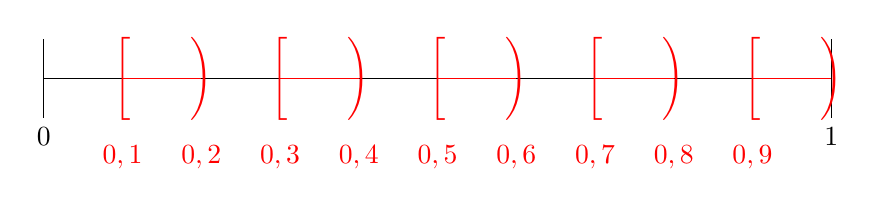
\begin{tikzpicture}
            \draw (0,0)-- (10,0); %Axis

            \draw (0,0.5) -- (0,-0.5) node[below] {0};
            \draw (10,0.5) -- (10,-0.5) node[below] {1};

            \node[red] at (1,-1) {$0,1$};
            \node[red] at (1,0) {$\Bigg[$};

            \node[red] at (2,-1) {$0,2$};
            \node[red] at (2,0) {$\Bigg)$};

            \node[red] at (3,-1) {$0,3$};
            \node[red] at (3,0) {$\Bigg[$};

            \node[red] at (4,-1) {$0,4$};
            \node[red] at (4,0) {$\Bigg)$};

            \node[red] at (5,-1) {$0,5$};
            \node[red] at (5,0) {$\Bigg[$};

            \node[red] at (6,-1) {$0,6$};
            \node[red] at (6,0) {$\Bigg)$};

            \node[red] at (7,-1) {$0,7$};
            \node[red] at (7,0) {$\Bigg[$};

            \node[red] at (8,-1) {$0,8$};
            \node[red] at (8,0) {$\Bigg)$};

            \node[red] at (9,-1) {$0,9$};
            \node[red] at (9,0) {$\Bigg[$};

            \node[red] at (10,0) {$\Bigg)$};

            \draw[red] (1,0)-- (2,0);
            \draw[red] (3,0)-- (4,0);
            \draw[red] (5,0)-- (6,0);
            \draw[red] (7,0)-- (8,0);
            \draw[red] (9,0)-- (10,0);
        \end{tikzpicture}
    \end{figure}
    % TODO weitere Intervalle
\end{auf}


\begin{auf}
    \subsubsection*{Berechnen Sie die Wahrscheinlichkeiten dieser Ereignisse.}
    \paragraph{Lösung:}
    Für 1.
    \[
        \pe(A_1) = \pe (\bigsqcup^5_{k=1} [\frac{2k-1}{10}, \frac{2k}{10})) = \sum^5_{k=1} \pe([\frac{2k-1}{10}, \frac{2k}{10}))
        = \sum^5_{k=1} \pe([\frac{1}{10}, \frac{2}{10})) = 5 \dot \pe([\frac{1}{10}, \frac{2}{10})) = 5 \cdot \frac{1}{10} = \frac{1}{2}
    \]
    Für 2.
    \[
        \pe(A_2) = \sum^9_{i=0} \pe([\frac{10i + 4}{100}, \frac{10i + 5}{100})) = 10 \cdot \frac{1}{100} = \frac{1}{10}
    \]
    Für 3.
    \[
        \pe(A_3) =  \sum^5_{i=0} \pe([ \frac{10i+(5-i)}{100}, \frac{10i+(5-i)+1}{100})) = 6 \cdot \frac{1}{100} = \frac{3}{50}
    \]
    Für 4. WS für Einpunktmenge bei Dichte ist 0 = $\int_{1/\pi}^{1/\pi} 1 \dx = \frac{1}{\pi} - \frac{1}{\pi}$ \\
    % TODO das mit den Punktmengen einerseits in den Index, andererseits irgendwie nochmal im Skript einfügen
    Für 5.
    \[
        \pe(A_5) = \pe([\frac{1}{\pi}-\frac{1}{100}, \frac{1}{\pi} + \frac{1}{100}]) = \frac{2}{100}
    \]
\end{auf}